\subsection{Beweistheorie der Aussagenlogik}
\subsubsection{Typische Fragestellungen}
\begin{itemize}
	\item Ist $F$ Tautologie?
	\item Ist $G$ erfüllbar? \qquad ( Ist $G$ Tautologie? )
	\item Gilt $A_1 , \dotsc , A_n \models B$ \quad (= Ist $A_1 \wedge \dotsb \wedge A_n \rightarrow B$ Tautologie? = \\
		Ist $A_1 \wedge \dotsb \wedge A_n \wedge B$ unerfüllbar?)
\end{itemize}
\begin{bsp}
	\begin{gather*}
		F = \bigwedge_{i=1}^n ( \bigvee_{j=1}^{m_i} L_{ij} ) \qquad \text{Ist } F \text{ Tautologie?} \\
		F = F_1 \wedge \dotsb \wedge F_n \\
		F \text{ Tautologie, \gdw } F_1 , \dotsc , F_n \text{ Tautologien} \\
		\begin{split}
			& F_1 = L_{1,1} \vee \dotsb \vee F_{1,m_1} \text{ Tautologie, \gdw für eine Atomformel } A \\
			& \text{ sowohl } A \text{ als auch } \neg A \text{ in } F_1 \text{ vorkommen.}
		\end{split}
	\end{gather*}
\end{bsp}
\begin{bsp}
	\begin{gather*}
		\begin{array}{ l l }
			F = \bigvee_{i=1}^n ( \bigwedge_{j=1}^{m_i} L_{ij} )		& \text{Ist } F \text{ Tautologie?} \\
			F = F_1 \vee \dotsb \vee F_n					& \text{nicht \enquote{lokalisierbar}}
		\end{array}
	\end{gather*}
	Offensichtliche Methode: Wahrheitstabelle. \\
	\begin{tabular}{ l l}
		Unterschied? \\
		Formel $F$ der Länge $l$			\\
		Bsp. 1: 	& \# Schritte $\sim l$		\\
		Bsp. 2: 	& \# Schritte $\sim 2^l$
	\end{tabular}
\end{bsp}

\subsubsection{Kleiner Ausflug in die Komplexitätstheorie}
Frage (Input) $\rightarrow$ Algorithumus $\rightarrow$ Antwort (Output) \\
Interessante Grösse: \# Schritte (Länge des Inputs $l$) = $T( l ) \leq f( l )$ \quad worst-case \\
\begin{bsp*}
	\begin{tabular}{ l l }
		$T( l ) \leq C_1$			& Was ist der n-te Bit?														\\
		$T( l ) \leq C_2 \cdot l$	& Addition, Tautologie für KNF												\\
		$T( l ) \leq C_3 \cdot l^2$	& Multiplikation ( zwar gibt es einen Algorithmus dafür \\&mit $T( l ) \leq C_4 \cdot l \cdot log l$	\\
		$T( l ) \leq C \cdot l^d$	& ( $c$ , $d$ Konstanten ) polynomiale Laufzeiten										\\
		$T( l ) \leq C \cdot 2^l$	& exponentielle Laufzeit z.B. Wahrheitstabelle aufstellen.								\\
		$T( l ) \leq 2^{^3\sqrt{l}}$	& subexponentiell - bester Bekannter Algorithmus \\&zur Primzahlzerlegung					
	\end{tabular}
\end{bsp*}
Komplexitätsklassen
P: Probelme, die polynomialer Zeit lösbar sind. \\
NP: Probleme, für die ein Lösungskandidat in polynomialer Zeit überprüfbar. \\
Niemand weiss, ob P $\neq$ NP gilt. \\ \todo{? Once wanted to do something here, but forgot what...}
NP-vollständig (NPC): schwierigste Probleme in NP: Polynomialer Algorithums für ein NPC $\rightarrow$ Polynomialer Algorithmus für jedes NP \\
\\
P $\ni$ Tautologieproblem für KNF \\
NP $\ni$ Tautologieproblem für DNF \\
\\
$F$ Tautologie \gdw $\neg F$ unerfüllbar \\
\begin{align*}
	F		& = \bigwedge_i F_i = \bigwedge_i ( \bigvee_i L_{ij} )	& \text{Tautologieproblem für KNF =} \\
	\neg F	& = \neg \bigwedge_i ( \bigvee_i L_{ij} ) = \bigvee_i ( \neg \bigvee_i L_{ij} ) = \bigvee_i ( \bigwedge_i  ( \neg L_{ij ) } ) & \text{(Un)erfüllbarkeitsproblem für DNF}\\
	F		& = \bigvee_i F_i = \bigvee_i ( \bigwedge_i L_{ij} )		& \text{Tautologieproblem für DNF =} \\
	\neg F	& = \neg \bigvee_i ( \bigwedge_i L_{ij} ) = \bigwedge_i ( \neg \bigwedge_i L_{ij} ) = \bigwedge_i ( \bigvee_i  ( \neg L_{ij ) } ) & \text{(Un)erfüllbarkeitsproblem für KNF =} \\
	&& \text{Umwandlung DNF } \leftrightsquigarrow \text{ KNF} \\
\end{align*}
Theorem (Cook 1971): \\
3-SAT ist in NPC \\
3-SAT: \\
Ist $( \dotsb \vee \dotsb \vee \dotsb ) \wedge ( \dotsb \vee \dotsb \vee \dotsb ) \wedge \dotsb \wedge ( \dotsb \vee \dotsb \vee \dotsb )$ erfüllbar?

\subsubsection{Was sind typische alltägliche Probleme?}
\begin{bsp*}[note = Sudoku]
	Bedingungen: $B_1 \wedge \dotsb \wedge B_n$ \\
	Frage: Gibt es eine Lösung? \\
	$\drsh$ KNF-Erfüllbarkeitsproblem \\
	$\drsh$ Sudoku ist NPC
\end{bsp*}

\subsubsection{Resolution: Unerfüllbarkeitsproblem für KNF}
Ist das Problem genug allgemein? \\
\begin{bsp*}
	$A_1 , A_2 , \dotsc , A_n \models B$ \quad gleichbedeutend mit $A_1 \wedge A_2 \wedge \dotsb \wedge A_n \wedge \neg B$
\end{bsp*}

\subsubsection{Mengenschreibweise für KNF-Formeln}
Mengen:
\begin{itemize}
	\item $A = \{ 1 , 2 , 12 \} = \{ 2 , 1 , 12 , 12 \}$
	\item $\varnothing = \{\}$
	\item $A \cup B$
	\item $A \cap B$
	\item $A \setminus B$
	\item \{ \{ 1 , 2 \} , \{ 3 , 4 , 5 \} \}
\end{itemize}
\begin{bsp*}
	\begin{gather*}
		F = \underbrace{\overbrace{( A \vee B \vee C )}^{\text{Klausel}}}_{\{ A , B , A \}} \wedge \underbrace{( B \vee \neg C )}_{\{ B , \neg C \}} \wedge \underbrace{( B \vee A )}_{\{B , A\}} \\
		\begin{aligned}
		F 	&= \{ \{ A , B , A \} , \{ B , ¬ C \} , \{ B , A \} \} \\
			&= \{ \{ A , B \} , \{ B , ¬ C \} , \{ B , A \} \} \\
			&= \{ \{ A , B \} , \{ B , ¬ C \} \}
		\end{aligned}
	\end{gather*}
\end{bsp*}
\begin{bsp*}
	\begin{gather*}
		A , A \rightarrow B , B \rightarrow C , C \rightarrow D , D \rightarrow E \models E \\
		\intertext{ist gleichbedeutend mit}
		A \wedge ( A \rightarrow B ) \wedge ( B \rightarrow C ) \wedge ( C \rightarrow D ) \wedge ( D \rightarrow E ) \wedge \neg E \\
		\text{ ist unerfüllbar} \\
		\{ \{ A \} , \{ \neg A , B \} , \{ \neg B , C \} , \{ \neg C , D \} , \{ \neg D , E \} , \{ \neg E \} \}
	\end{gather*}
	Es gibt keine Belegung, die alle Klausel erfüllt. \\
	Indirekt: Es gibt eine Belegung. \\
	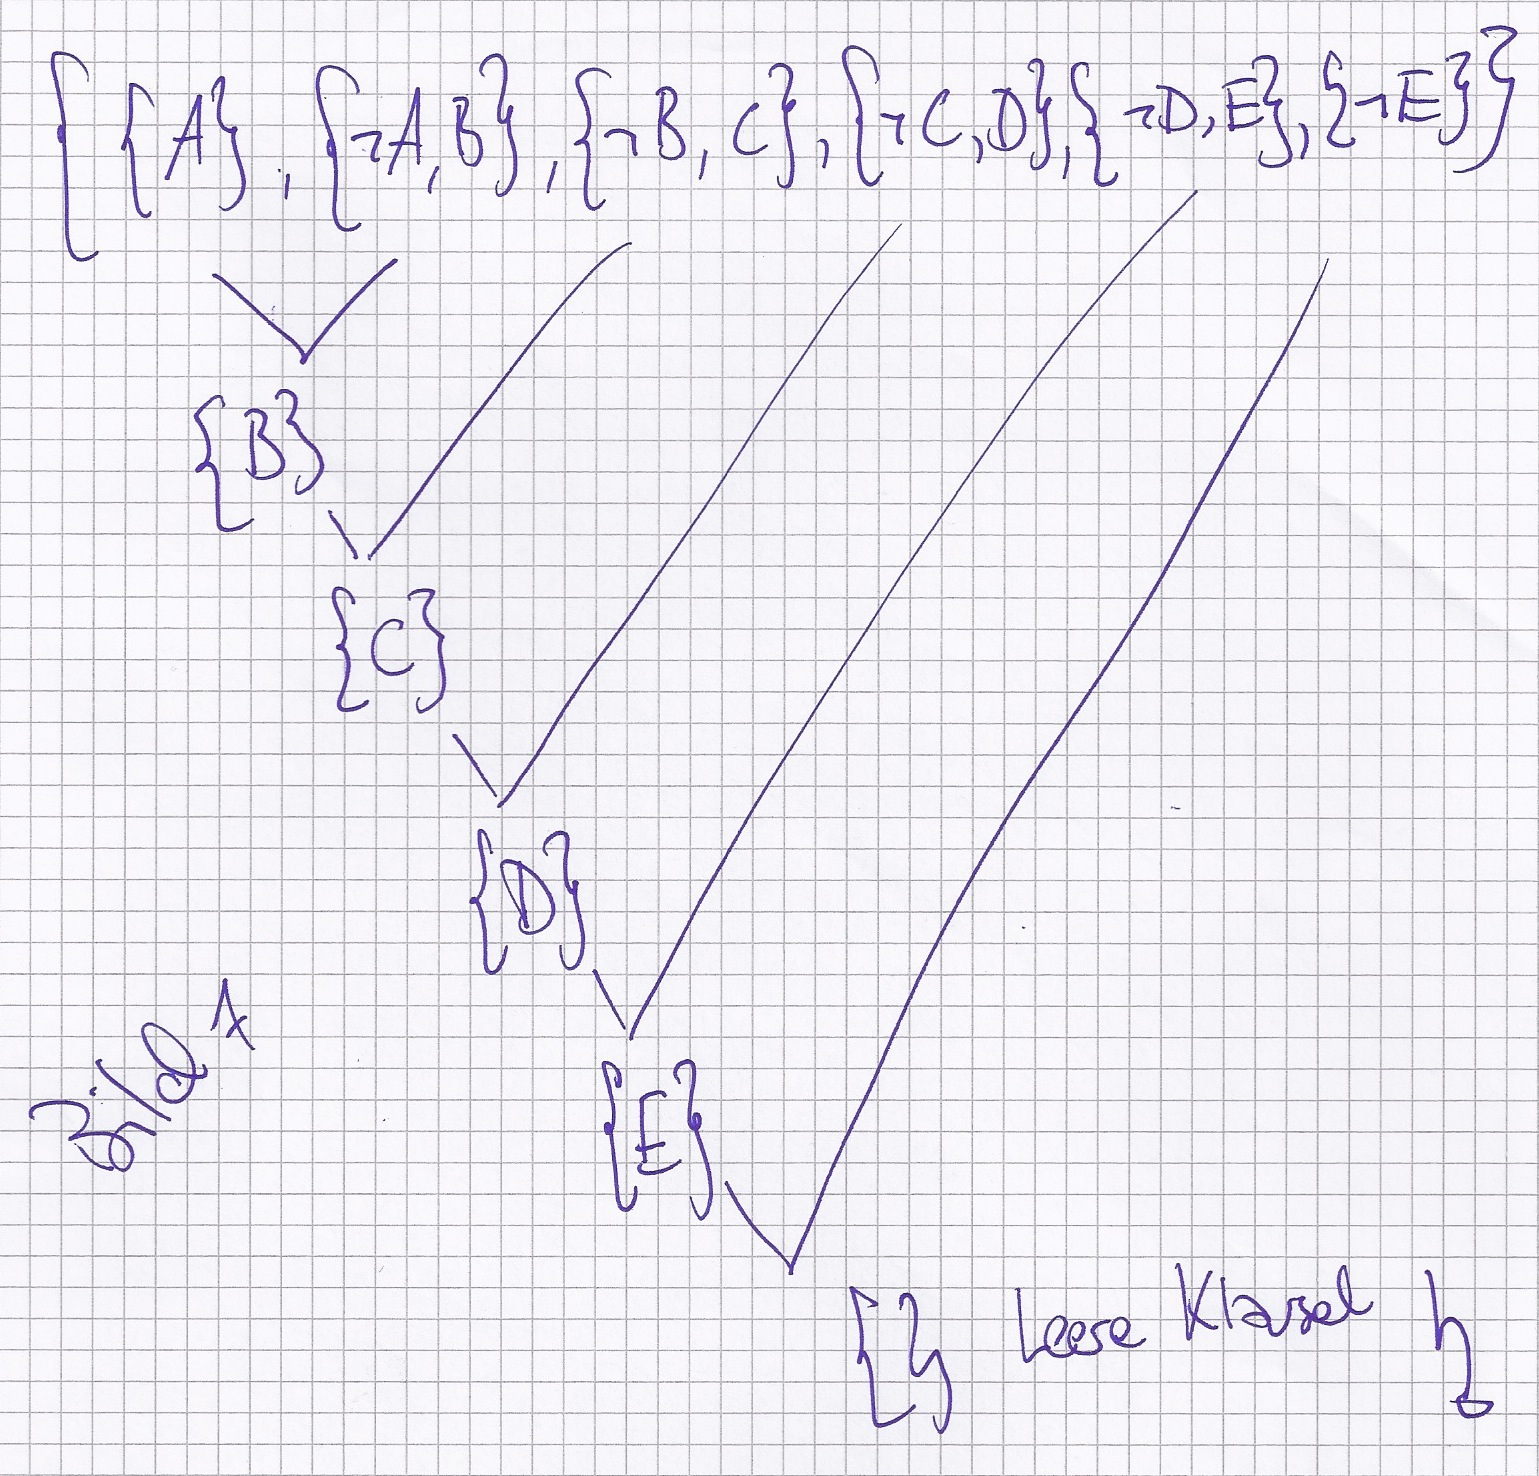
\includegraphics[width=\textwidth]{Bild9}
\end{bsp*}
\begin{bsp*}
	\begin{gather*}
		A \vee B , A \rightarrow C , B \rightarrow C \models C \\
		( A \vee B ) \wedge ( A \rightarrow C ) \wedge ( B \rightarrow C ) \wedge \neg  C \\
		\{ \{ A , B \} , \{ ¬ A , C \} , \{ ¬ B , C \} , \{ ¬ C \} \}
	\end{gather*}
	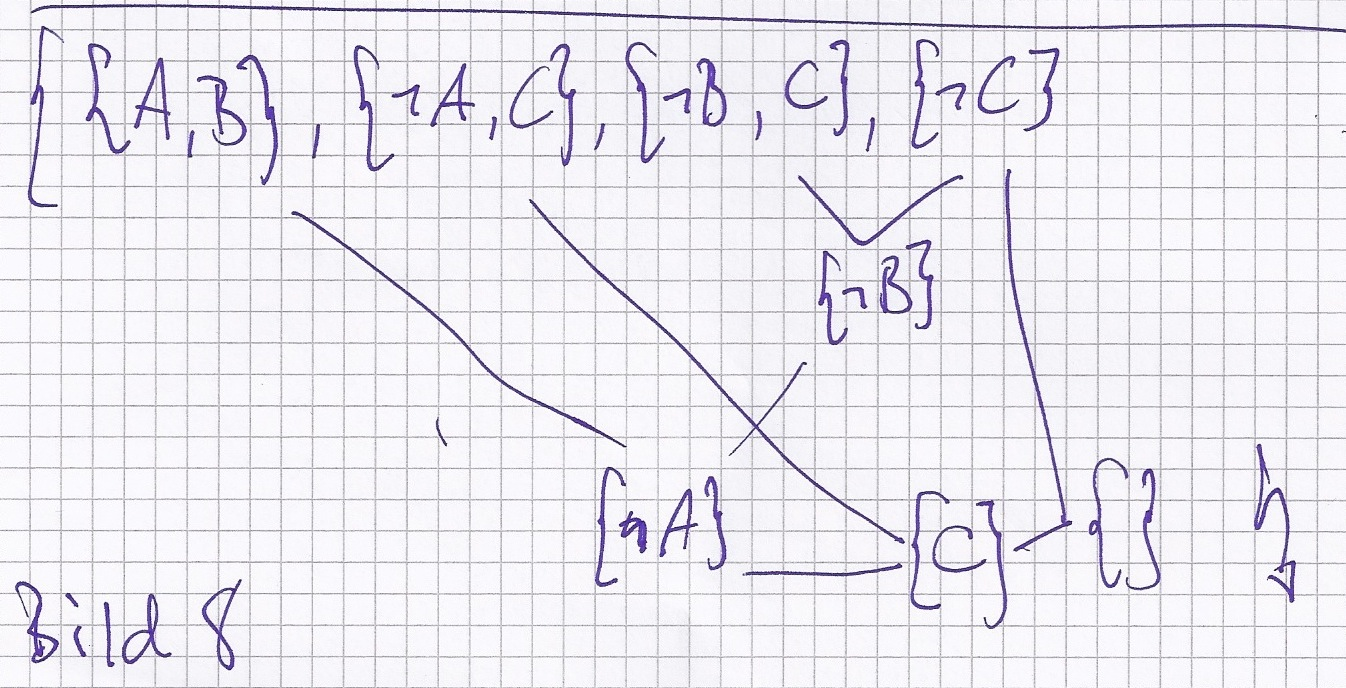
\includegraphics[width=\textwidth]{Bild10}
\end{bsp*}
\begin{bsp*}
	Der entscheidende Schritt: \\
	Jede Belegung die sowohl \\
	$\{ \underset{\uparrow}{A} ,  B , \neg C \}$ als auch $\{ \underset{\uparrow}{\neg A} , \neg E \}$ wahr macht,\\
	muss auch $\{ B , \neg C , \neg E \}$ erfüllen. \\
	Wieso?\\
	\[\begin{array}{ l l l l }
		\text{Fall 1:}	& \mathcal{A}( A ) = 0	& \text{Dann } \{ B , \neg C \} \text{ wahr,}	& \text{also auch } \{ B , \neg C , \neg E \}	\\
		\text{Fall 2:}	& \mathcal{A}( A ) = 0	& \text{Dann } \{ \neg E \} \text{ wahr,}		& \text{also auch } \{ B , \neg C , \neg E \}	
	\end{array}\]
\end{bsp*}
\begin{def*}[note = Resolvent , index = Resolvent]
	$K_1 , K_2 , R$ Klauseln \\
	$\mathbf{R}$ \textbf{Resolvent} von $K_1$ und $K_2$, falls es ein Literal $L$ gibt mit $L \in K_1$ und $\neg L \in K_2 , \mathbf{R=( K_1 \setminus \{ L \} ) \cup ( K_2 \setminus \{ \neg L \} )}$
\end{def*}
\begin{satz*}
	$R$ Resolvent von $K_1 , K_2$. Dann
	\[K_1 , K_2 \models R\]
	Beweis: Übung
\end{satz*}
\begin{bsp*}
	$$F = ( A \vee B \vee \neg C ) \wedge ( \neg A \vee \neg E ) \wedge ( \neg C \vee D \vee E ) \wedge C \wedge ( \neg D \vee \neg C )$$
	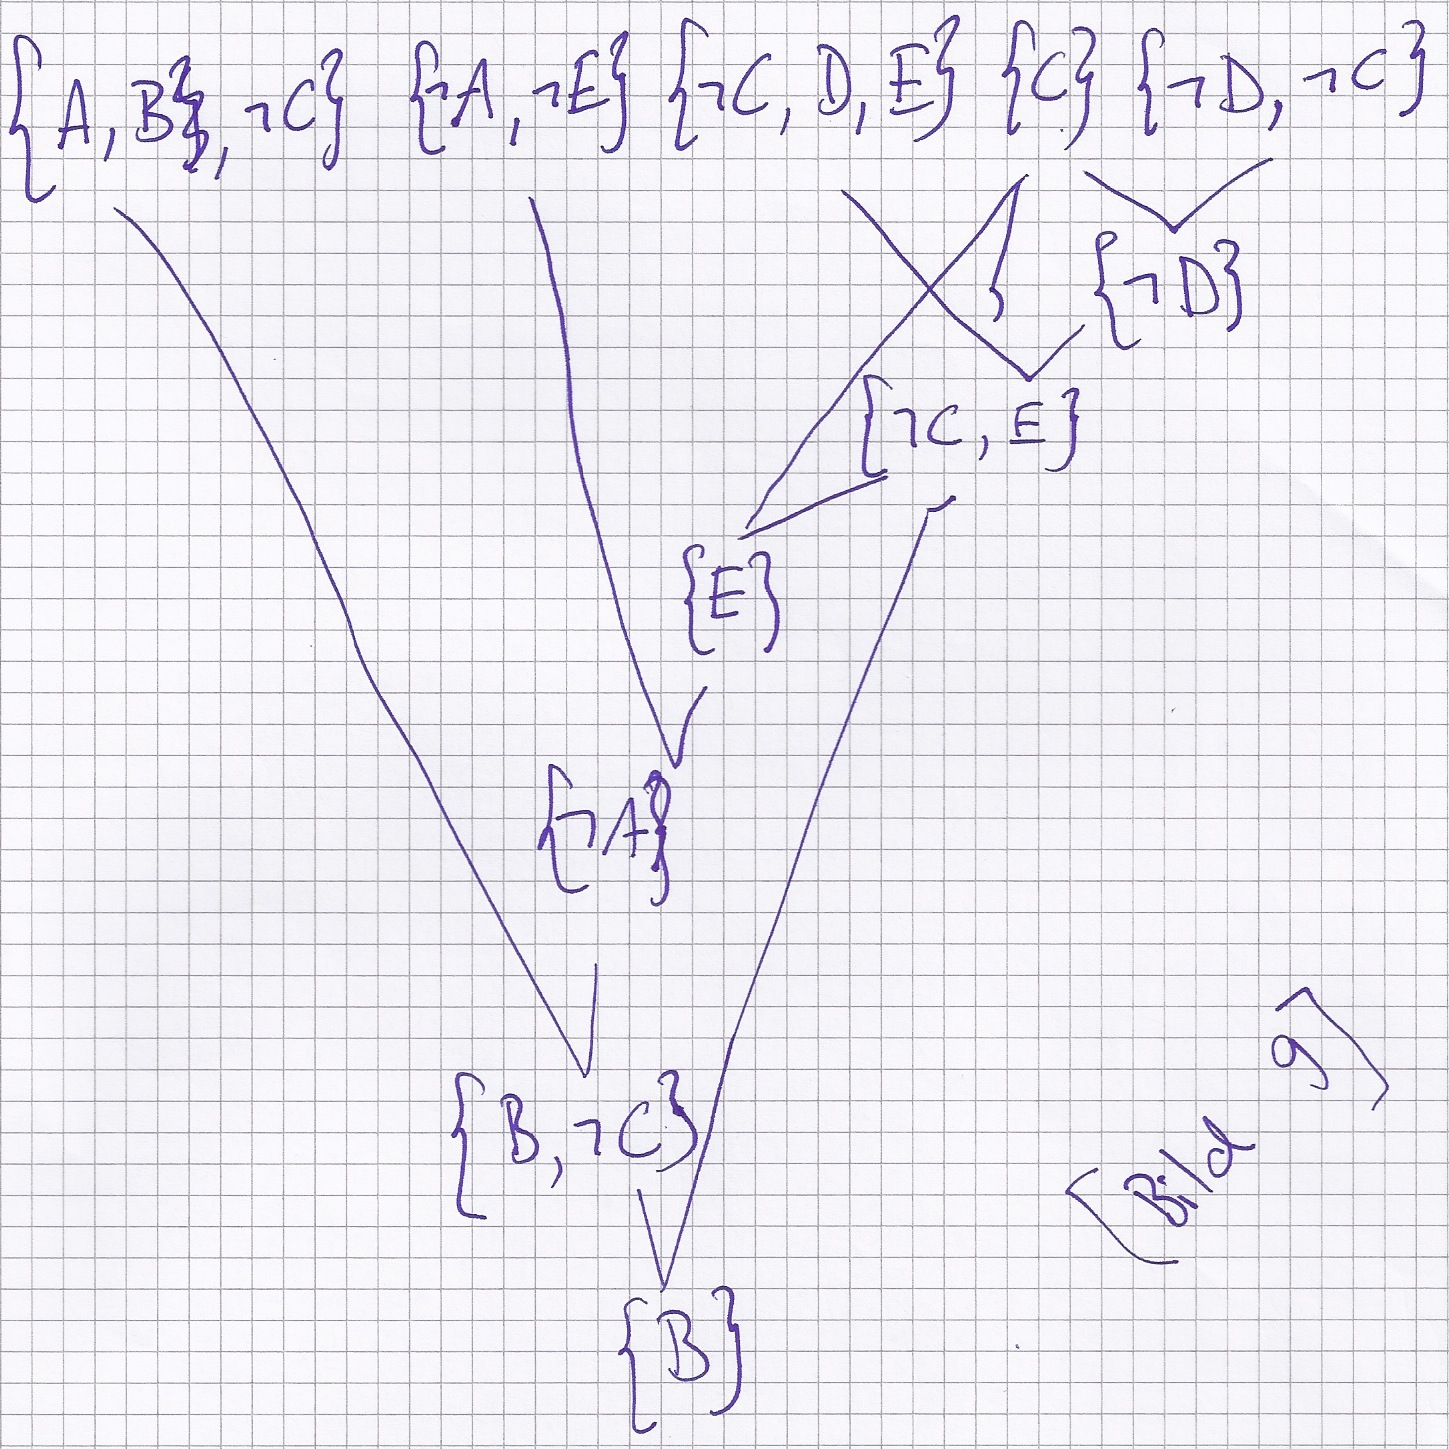
\includegraphics[width=\textwidth]{Bild11}\\
	\begin{itemize}
		\item $\{\}$ lässt sich nicht resolvieren.
		\item F ist erfüllbar und zwar durch $\mathcal{A}( A ) = 0 , \mathcal{A}( B ) = 1 ,$ \\
			$\mathcal{A}( C ) = 1 , \mathcal{A}( D ) = 0 , \mathcal{A}( E ) = 1$
		\item Es gibt keine andere erfüllende Belegung.
	\end{itemize}
\end{bsp*}
\begin{bsp*}
	$F \coloneqq ( \neg B \wedge C \wedge D ) \vee ( \neg B \wedge \neg D ) \vee ( C \wedge D ) \vee B$ \\
	Ist $F$ Tautologie? \\
	Ist $\neg F$ unerfüllbar? \\
	\begin{bew}
		$\neg F \equiv ( B \vee C \vee \neg D ) \wedge ( B \vee D ) \wedge ( \neg C \vee \neg D ) \wedge \neg B$ \\
		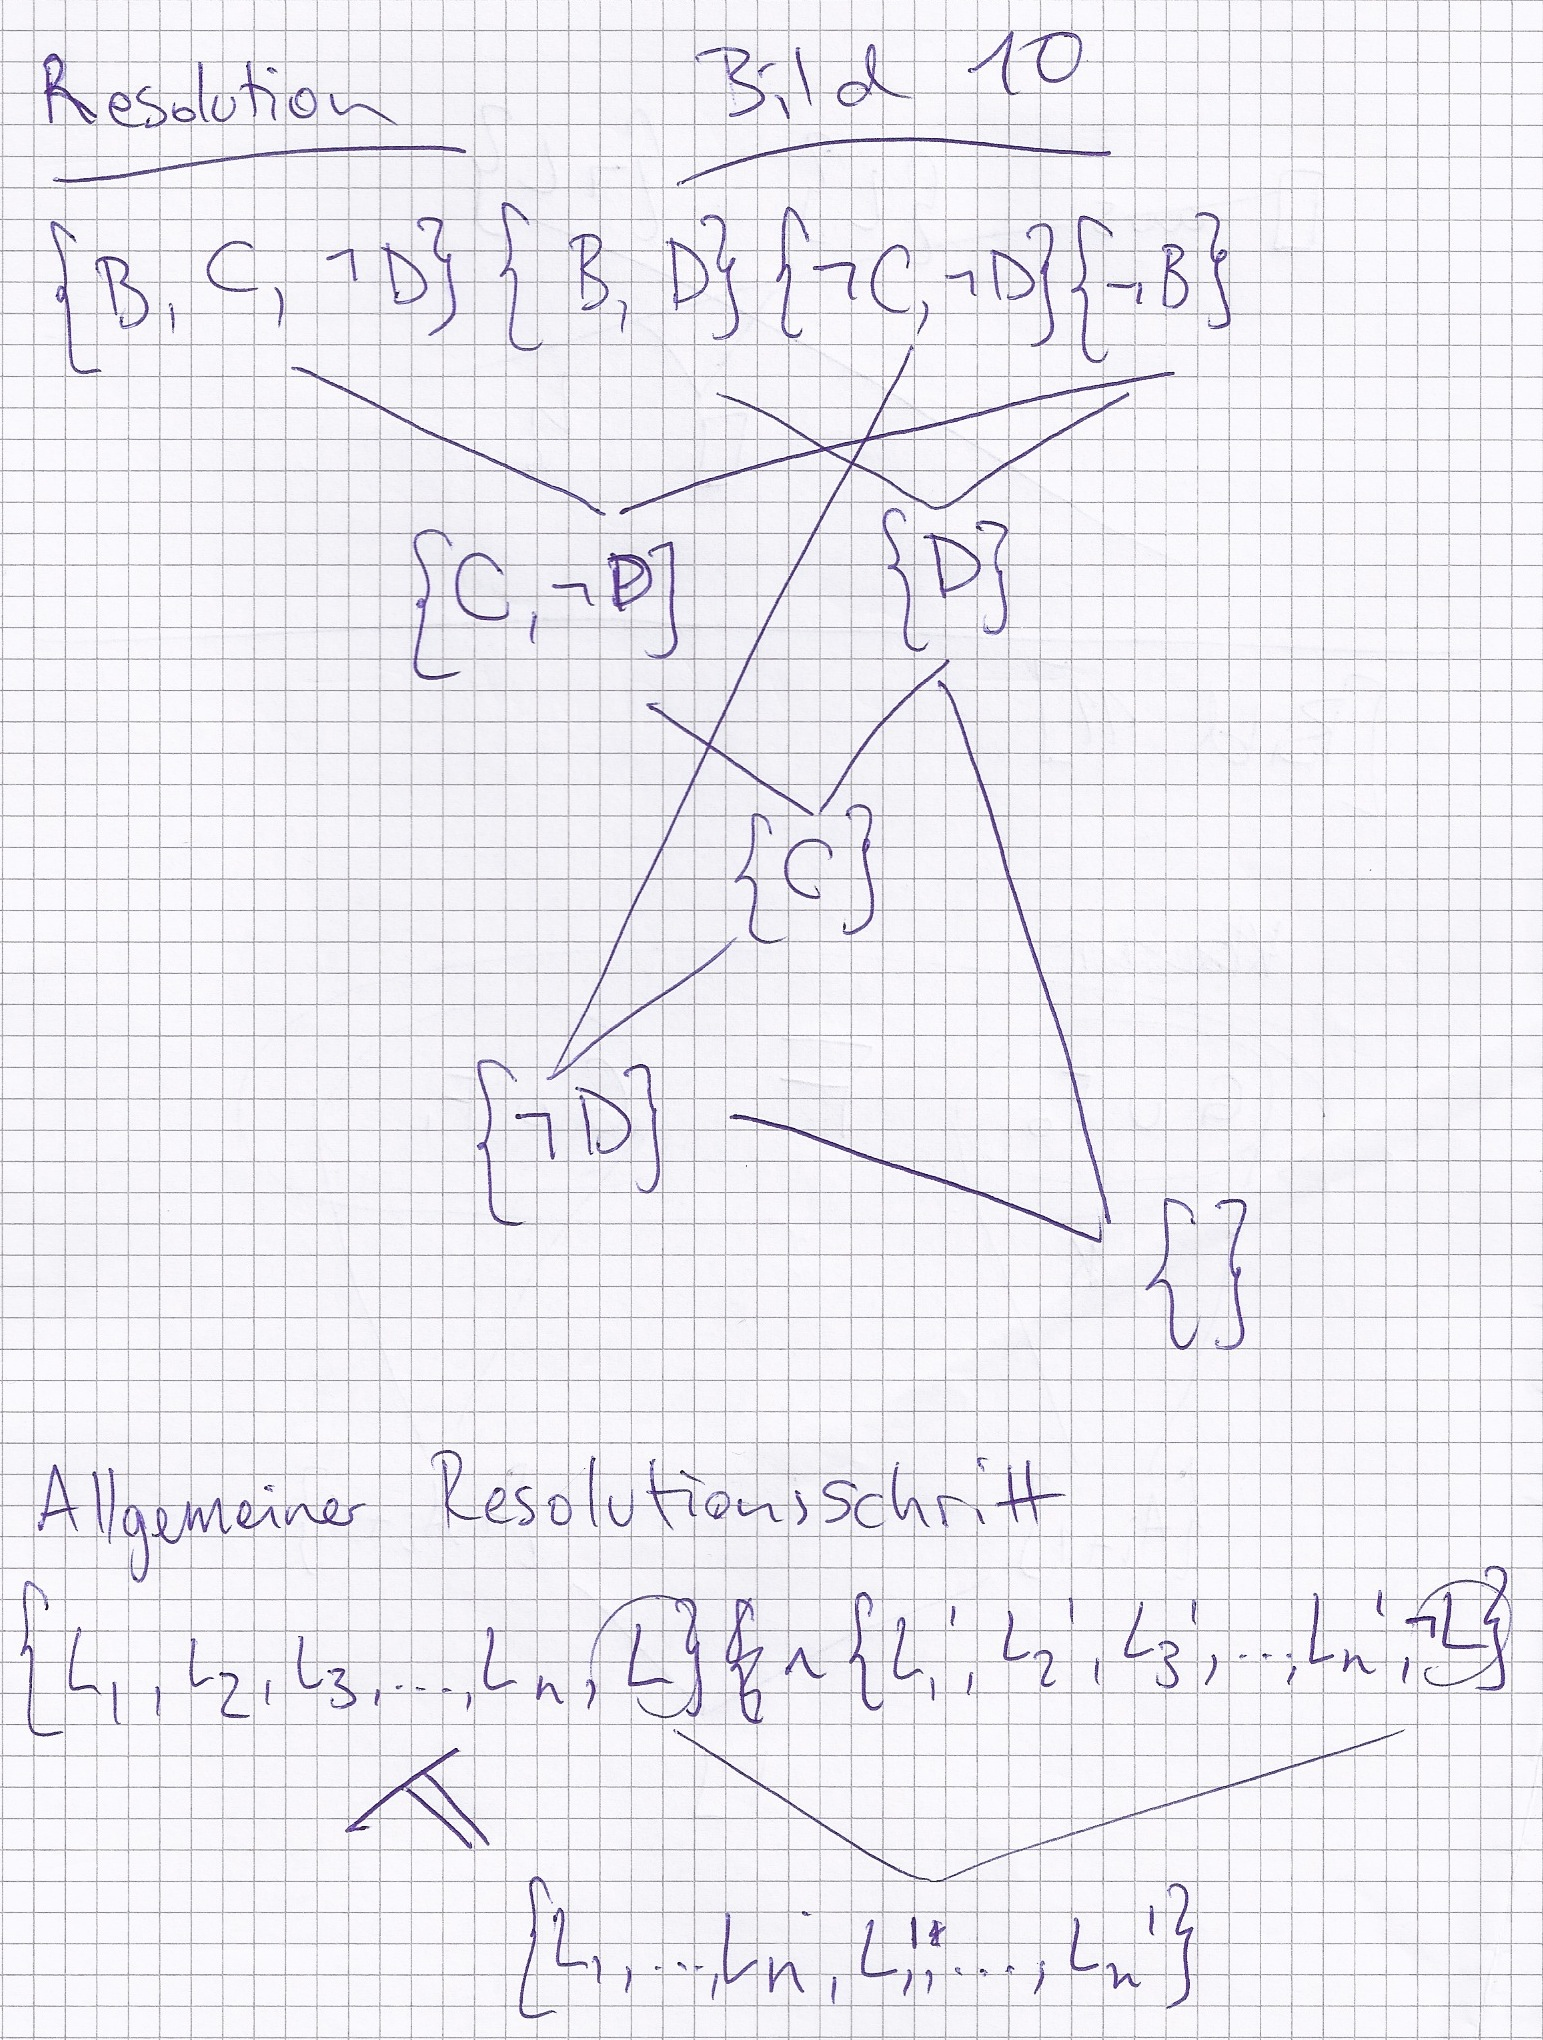
\includegraphics[width=\textwidth]{Bild12}
	\end{bew}
\end{bsp*}

\subsubsection{Was wollen wir von einem Beweiskalkül?}
\begin{description}
	\item[Korrektheit:] \enquote{nichts falsches beweisbar}.
	\begin{itemize}
		\item $F \rightsquigarrow \{\}$, dann $F$ unerfüllbar.
	\end{itemize}
	\item[Vollständigkeit:] \enquote{alles richtige bewiesbar}.
	\begin{itemize}
		\item $F$ unerfüllbar, dann $F \rightsquigarrow \{\}$.
	\end{itemize}
	\item[Effizienz:] Problem: NP-vollständig
	\item[Termination:] bricht ab
\end{description}
$F$ Formel in KNF, Klauselmenge \\
$\Res( F ) \coloneqq \{ \text{Resolvent } R \text{ zweier Klauseln } K_1 , K_2 \text{ in } F \} \cup F$ \\
Dann $\Res( F ) \equiv F$\\
\begin{enumerate}
	\item Prozess $F \rightarrow \Res( F ) \rightarrow \Res( \Res( F ) \rightarrow \dotsb \rightarrow \Resf( F )$ bricht ab.
	\item Falls $F$ unerfüllbar, dann $\Box = \{\} \in \Resf( F )$
\end{enumerate}
\begin{enumerate}
	\item Weil es über einem endlichen Alphabet ( =Atomformeln ) nur endlich viele Klauseln gibt ( als Mengen  ): Nämlich $3^n \text{ über } A_1 , \dotsc , A_n$
	\item Theorem( Hauptsatz der Resolution ) $F$ ist unerfüllbar \gdw $\Box \in \Resf( F )$
	\begin{itemize}
		\item
			\begin{bew}
				$\enquote{\Leftarrow} \Box \text{ aus } \{ L \} \{ \neg L \} \: \text{\lightning}$
			\end{bew}
		\item
			\begin{bew}
				$\enquote{\Rightarrow} \text{ Induktion über Anzahl } n \text{ Atomformeln}$
				\begin{itemize}
					\item Verankerung $n=1$ \\
					\begin{gather*}
						\begin{array}{ l l }
							F \equiv \{ \{ A_1 \} \}									\\
							F \equiv \{ \{ \neg A_1 \} \}								\\
							F \equiv \{ \{ \} \}  = \{ \Box \}							\\
							F \equiv \{ \{ A_1 \} \{ \neg A_1 \} \}	& (A_1 \wedge \neg A_1 )	\\
							F \equiv \{ \{ A_1 , \neg A_1 \} \}		& ( A_1 \vee \neg A_1 )	
						\end{array}
					\end{gather*}
					\item Induktionvoraussetzung:
					\begin{itemize}
						\item Richig für $A_1 , \dotsc , A_i$
					\end{itemize}
					\item Induktionsschritt:
					\begin{itemize}
						\item Richtig für $A_1 , \dotsc , A_{i+1}$
						\item $G$ Klauseln ohne $A_{i+1} , \neg A_{i+1}$
						\item
							\begin{gather*}
								F_0 \text{ Klauseln mit } A_{i+1} \\
								F_1 \text{ Klauseln mit } \neg A_{i+1} \\
								F_0' \coloneqq \{ K \setminus \{ A_{i+1} \} \mid K \in F_0 \} \\
								F_1' \coloneqq \{ K \setminus \{ A_{i+1} \} \mid K \in F_1 \}
							\end{gather*}
						\item
							\begin{description}
								\item[Fall 1:] $G \text{ unerfüllbar } \implies \Box \in \Resf( G ) \implies \Box \in \Resf( F )$
								\item[Fall 2:] $G \text{ erfüllbar. Es gilt } G \cup F_0' \text{ unerfüllbar}$
								\begin{itemize}
									\item Indirekt. $G \cup F_0'$ erfüllbar.
									\begin{gather*}
										\text{Belegung } \mathcal{A}\{ A_1 , \dotsc , A_i \} \rightarrow \{ 0 , 1 \} \\
										\text{Zusätzlich } \mathcal{A}( A_{i+1} ) = 0 \\
										\mathcal{A} \text{ erfüllt: } G , F_0 , F_1 , \text{ also F \lightning  Theorem }
									\end{gather*}
									\item Analog $G \cup F_1'$ unerfüllbar
								\end{itemize}
							\end{description}
					\end{itemize}
					\item Induktionsvoraussetzung: \\
						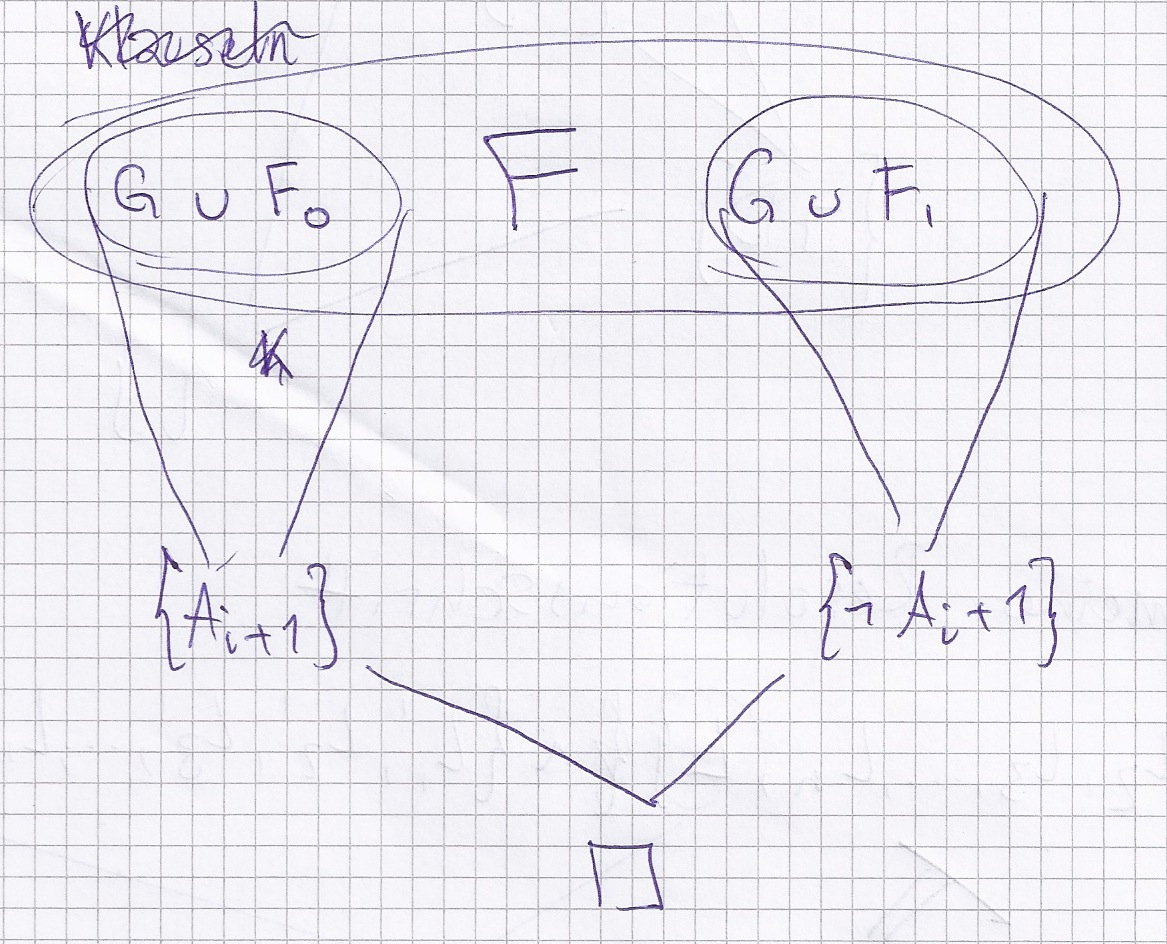
\includegraphics[width=\textwidth]{Bild13}
				\end{itemize}
			\end{bew}
	\end{itemize}
\end{enumerate}
\todo{Vertical spacing}
\todo{Too long}

\subsubsection{Resolutionsalgorithmus}
\begin{algorithmic}
\REQUIRE $F$ in KNF
\REPEAT
	\STATE $G \coloneqq F$
	\STATE $F \coloneqq \Res( F )$
\UNTIL{ $\Box \in F$ or $F = G$}
\IF{ $\Box \in F$ }
	\PRINT \enquote{unerfüllbar}
\ELSE
	\PRINT \enquote{erfüllbar}
\ENDIF
\end{algorithmic}

\subsubsection{Effizienter Spezialfall: Hornlogik}
Hornformel: $A_1 \wedge A_2 \wedge \dotsb \wedge A_n \rightarrow B \equiv \{ \neg A_1 , \neg A_2 , \dotsc , \neg A_n , B \}$ \\
\begin{def*}[note = Hornformel , index = Hornformel]
	\textbf{Eine Hornformel hat höchstens ein positives (nicht-negatives) Literal.}
\end{def*}
\begin{bsp*}
	\begin{gather*}
		\left.\begin{array}{ l }
			\left.\begin{array}{ l l }
				A							& \{ A \}					\\
				B							& \{ B \}					\\
				C							& \{ C \}					
			\end{array} \right\} \textbf{Fakten}	\\
			\left.\begin{array}{ l l }
				A \wedge B \wedge E \rightarrow F	& \{ \neg A , \neg B , \neg E , F \}	\\
				C \wedge D  \rightarrow G			& \{ \neg C , \neg D , G \}		\\
				B \wedge C  \rightarrow D			& \{ \neg B , \neg C , G \}		\\
				G \wedge A  \rightarrow E			& \{ \neg G , \neg A , E \}		
			\end{array} \right\} \textbf{Regeln}
		\end{array} \right\} \textbf{Datenbank}	\\
		\text{Gilt } E \text{? (\gdw Datenbank } \cup \{ \neg E \} \text{ unerfüllbar ) } \textbf{Abfrage}
	\end{gather*}
\end{bsp*}
2 Approaches:
\begin{itemize}
	\item Markierungsalgorithumus (Bottom-up)
	\item Lineare Resolution (Top-down)
\end{itemize}
